\documentclass{article}

\usepackage[a4paper, total={6in, 8in}]{geometry}
\usepackage[utf8]{inputenc}
\usepackage{amsmath}
\usepackage{amssymb}
\usepackage{tabularx}
\usepackage[makeroom]{cancel}
\usepackage{arydshln}
\usepackage{graphicx}
\usepackage{fancyhdr}
\usepackage{enumitem}
\usepackage{multirow}
\usepackage{amsfonts}

\newcommand{\overbar}[1]{\mkern 1.5mu\overline{\mkern-1.5mu#1\mkern-1.5mu}\mkern 1.5mu}

\pagestyle{fancy}
\fancyhf{}
\lhead{John J Li}
\rhead{CSE120 Spring 2021 Homework 5}
\rfoot{\thepage}
\lfoot{April 2021} 
\renewcommand{\headrulewidth}{0.4pt}
\renewcommand{\footrulewidth}{0.4pt}

\setlength{\parskip}{1em}
\setlength\parindent{0px}
\title{CSE120 Spring 2021 Homework 5}
\date{\today}
\author{John J Li}

\begin{document}
    \maketitle
    \thispagestyle{empty}
    \noindent\rule{\textwidth}{0.8pt}

    %###################################################################################

    \section*{Problem 1}

    Problem 1: (5 pts) Draw the logic diagram for a circuit that has two T flip-flops with 
    results $Q_A$ and $Q_B$, two user controlled inputs X and Y, and one output Z specified by 
    the following input equations:
    \begin{align*}
        T_A=Q_B'(Q_A+Y)' \\
        T_B=X\oplus Q_A\oplus Y' \\
        Z=(Q_BX)'
    \end{align*}

    \textbf{Solution:}
    \begin{center}
        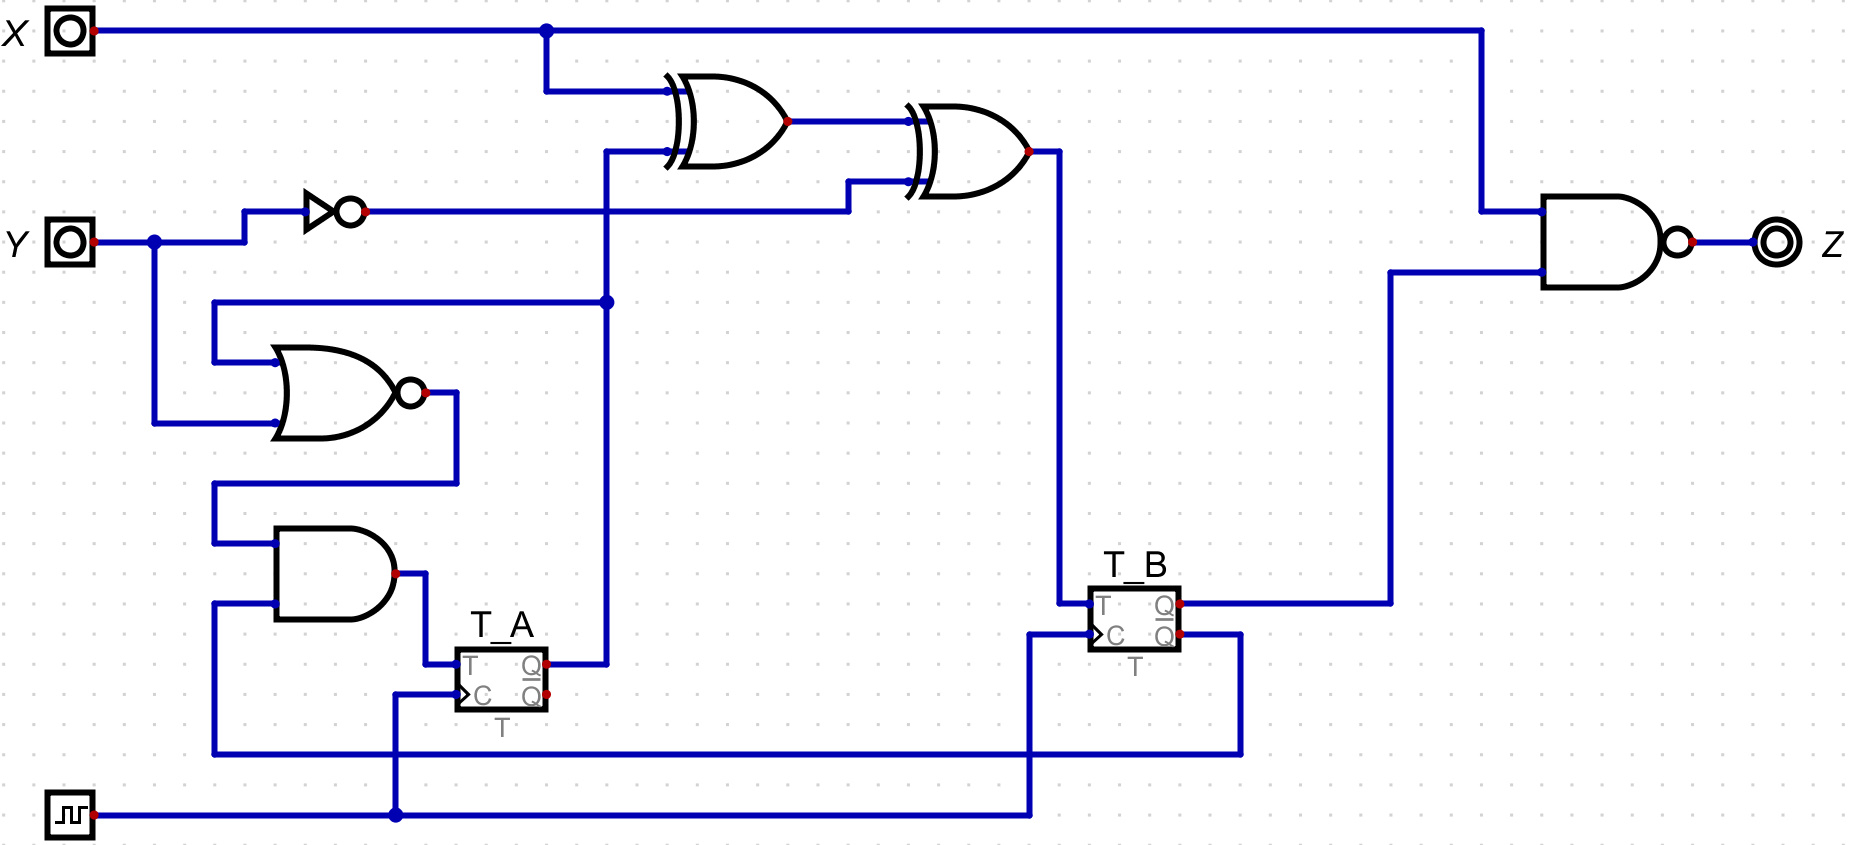
\includegraphics[width=\linewidth]{HW5_01_s01.jpg}
    \end{center}

    %###################################################################################

    \section*{Problem 2}

    For the collowing circuit, fill in the unshaded blank cells of the state table.

    \begin{center}
        \includegraphics[scale=1]{hw5_02_circuit.jpg}
    \end{center}

    \textbf{Solution:}

    \begin{center}
        \begin{tabular} {|c|c|}
           \hline 
           $J=x$ & \multirow{2}{8em}{$q_1^+=J\overbar{q_1}\lor\overbar{K}q_1$} \\
           $K=\overbar{x}\land \overbar{q_3}$ & \\
           \hline
           $S=\overbar{q_1}$ & \multirow{2}{8em}{$q_2^+=S\lor\overbar{R}q_2$} \\
           $R=q_1$ & \\
           \hline
           $D=x\lor q_2$ & $q_3^+=D$ \\
           \hline
        \end{tabular}
    \end{center}

    \begin{center}
        \begin{tabular} {|c|c|c|c|c|c|c|}
            \hline
            &\multicolumn{2}{c|}{$q_1^+$}&\multicolumn{2}{c|}{$q_2^+$}&\multicolumn{2}{c|}{$q_3^+$} \\
            \hline
            $q_1q_2q_3$ & $x=0$ & $x=1$ & $x=0$ & $x=1$& $x=0$ & $x=1$ \\
            \hline
            $000$ &0&1&1&1&0&1 \\
            $001$ &0&1&1&1&0&1 \\
            $010$ &0&1&1&1&1&1 \\
            $011$ &0&1&1&1&1&1 \\
            $100$ &0&1&0&0&0&1 \\
            $101$ &1&1&0&0&0&1 \\
            $110$ &0&1&0&0&1&1 \\
            $111$ &1&1&0&0&1&1 \\
            \hline
        \end{tabular}
    \end{center}
    
    %###################################################################################

    \section*{Problem 3}

    Design a synchronous machine (Transition Table, K-maps, Final Equations, Circuit 
    Diagram) that counts through the following sequence in the order shown 
    below. Note, there are no inputs or output variables, so your Q values must 
    reflect the Hex value listed.
    \begin{center}
        B 9 4 8 C A 3 0 and repeat
    \end{center}

    a) using all D flip-flops and combinational logic (AND/OR/NOT gates only)

    \textbf{Solution:}

    Transition Table:

    \begin{center}
        \begin{tabular} 
            
        \end{tabular}
    \end{center}

    b) using all T flip-flops and one multiplexer of size 8:1 per flip flop.

    %###################################################################################

    \section*{Problem 4}

    Use the following state transition diagram to answer the questions below:

    \begin{center}
        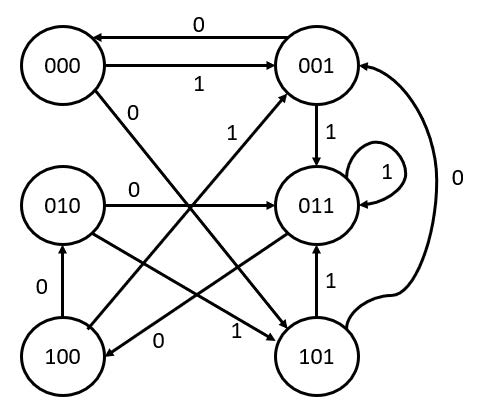
\includegraphics{HW5_04_StateDiagram.jpg}
    \end{center}

    a) How many flip flops are required to make this circuit? (1 pt)

    b) Given a starting state of 000, what is the shortest sequence of input values of X that would need to occur to end in state 010? (2 pts)

    c) Create the state transition table for this circuit. (5 pts)

    d) Create the circuit schematic for this design using only JK flip flops and any combinational logic (AND/OR/NOT gates only). (8 pts)

    e) What would be the next state if the starting state was 111 and the input X = 0? (2 pts)

    %###################################################################################

    \section*{Problem 5}

    Given the following state diagram with one input X and one output Z:

    \begin{center}
        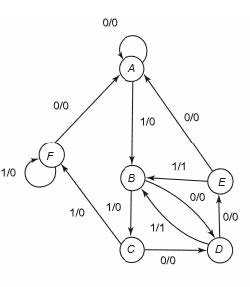
\includegraphics{HW5_05_StateDiagram.jpg}
    \end{center}

    a) Is this a Moore or Mealy machine? (1 pt)

    b) Create a state transition table. (3 pts)

    c) Complete the timing trace as far as possible given the following input: (3 pts)

    \begin{center}
        \begin{tabular}{|c|c|c|c|c|c|c|c|c|c|}
            \hline
            X & 0 & 1 & 1 & 0 & 1 & 1 & 1 & 1 & 0 \\
            \hline
            State & A &&&&&&&& \\
            \hline
            Z & 0 &&&&&&&& \\
            \hline
        \end{tabular}
    \end{center}

    %###################################################################################

    \section*{Problem 6}

    Design a synchronous lighted sign that flashes different colors based on an input L. 
    When L is equal to 0, the sign should flash the following sequence; blue, green, red, 
    and repeat. When L is equal to 1, the sign should flash the following sequence; yellow,
    off, red, off, yellow, off, red, off, and repeat. Assume the correct color will shine 
    when the associated state is present.

    If the sign is in the blue or green state and the input L should change to 1, the next 
    state should start the other sequence by transitioning to yellow first. If the sign is 
    in yellow, off, or red states and the input L changes to 0, the next state should start 
    the other sequence by transitioning to blue first.

    Create the State Definition Table, State Diagram, Transition Table, combinational logic 
    using Kmaps, and Final Equations assuming JK flip-flops and AND/OR/NOT combinational 
    logic.

    For any additional binary states that don't exist in your state transition diagram, 
    please solve for the next state using your JK equations and explain what the next state 
    would be if the input was 0 or if the input was 1.

    %###################################################################################

    \section*{Problem 1}
    %###################################################################################

    \section*{Problem 1}

\end{document}